\chapter{ECLAIR}\label{chapter:eclair}
ECLAIR is a powerful platform for software verification. At the moment of this writing the latest stable release, and the version adopted for the project described in Part~\ref{part:the-proof-of-concept}, is the 3.12.0.
Applications range from coding rule validation, with a particular emphasis on the MISRA and BARR-C coding standards, to the computation of software metrics, to the checking of independence and freedom from interference among software components, to the automatic detection of important classes of software errors.
ECLAIR is certified for use in safety-critical development ranging from automotive to aerospace use cases, moving to industrial and medical ones.
It uses formal methods-based static code analysis techniques such as abstract interpretation and model checking combined with constraint satisfaction techniques to detect or prove the absence of certain run time errors in source code, and provides support for program analysis and verification, program test generation and program transformation.

\begin{figure}[ht]
	\centering
	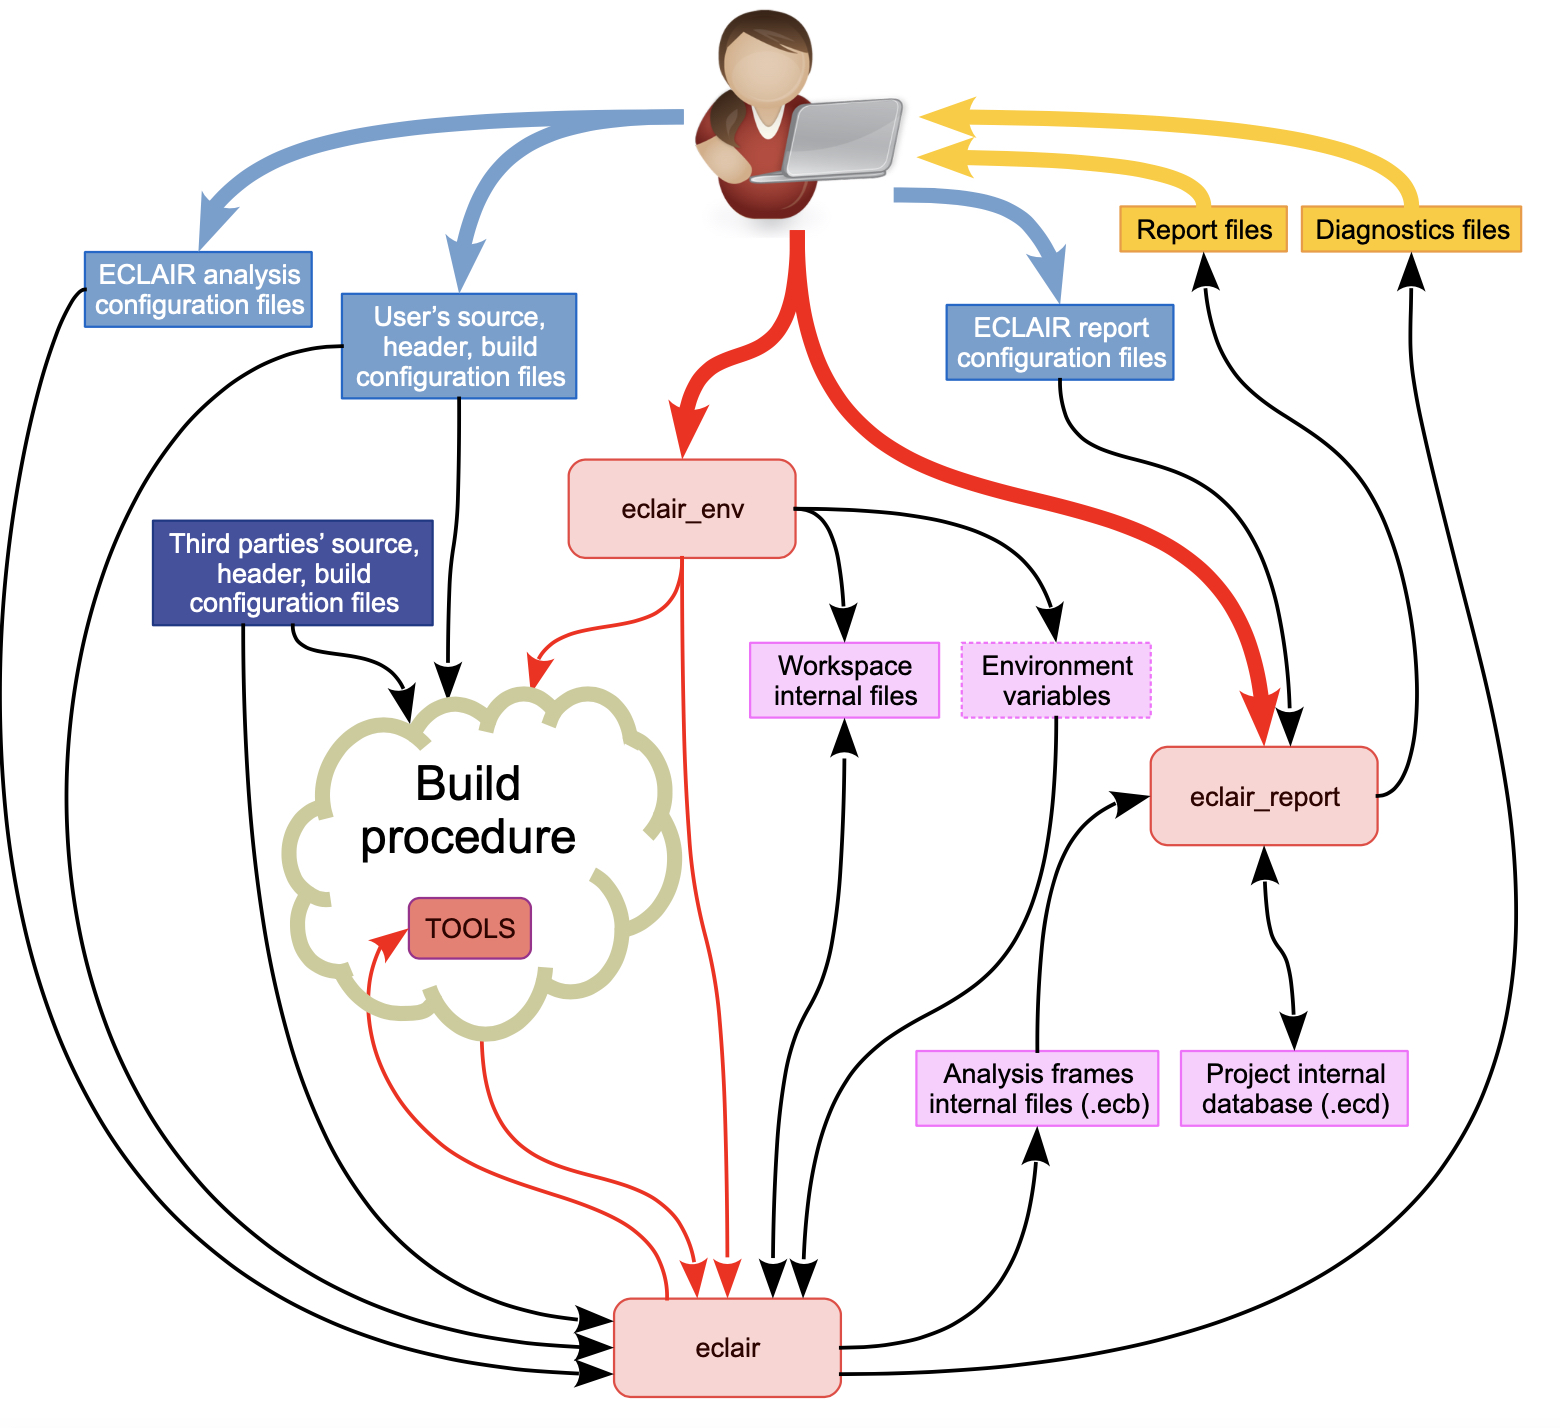
\includegraphics[width=1.0\textwidth]{Immagini/ECLAIR_basic_qualifiable_architecture.jpg}
	\caption{ECLAIR basic qualifiable architecture - Image copyright by BUGSENG srl, reproduced with permission.}
	\label{fig:one}
\end{figure}

\section{Abstract interpretation}
Abstract interpretation was formalized by the French computer scientists Patrick Cousot and Radhia Cousot in the late 1970s and it mainly consists of the automatic extraction of information about the possible execution paths of a program.
The formalization of all these possible execution paths is called \emph{concrete semantics}. The concrete semantics of a program is, in general, a non-computable, typically infinite mathematical object. Thus it is not possible to write a program to compute it. Having said that, all the non-trivial questions about the concrete semantics are undecidable. 

However, we can consider a sound approximation of the concrete program semantics, called \emph{abstract semantics}, and reason on it. Since the abstract semantics covers all possible cases, we can use it to demonstrate safety properties of the program.
\\\\
The abstract semantics is an artificial construct aimed at giving a computable approximation of the concrete semantics. It is important to pay attention to the ``direction'' of the approximation: it must ``err on the safe side'' in order to avoid false negatives, though at the expense of allowing false positives. 
However, once a good approximation is available, abstract interpretation can give precious insights into the program properties and inner workings. 

\begin{figure}[ht]
	\centering
	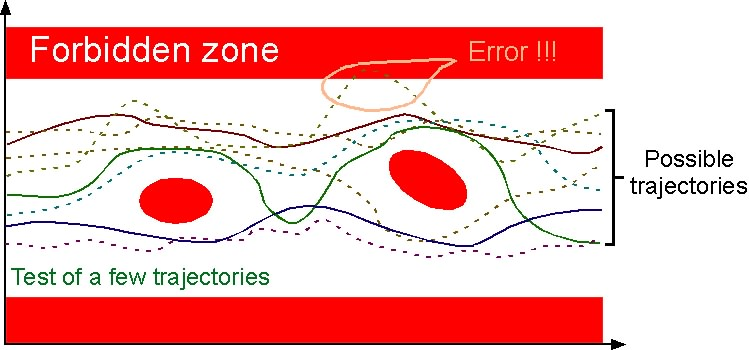
\includegraphics[width=1.0\textwidth]{Immagini/AbstractInterpretationNutshell_trajectories.jpeg}
  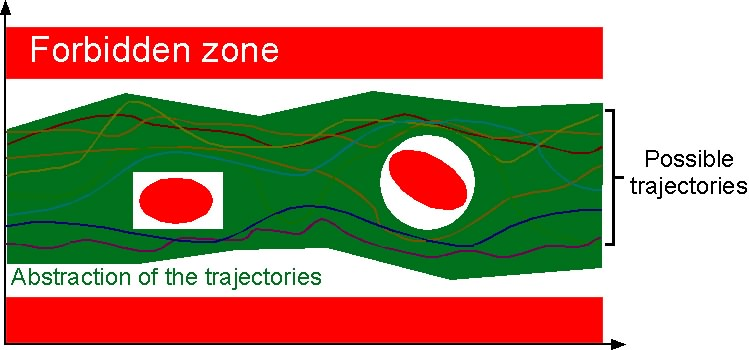
\includegraphics[width=1.0\textwidth]{Immagini/AbstractInterpretationNutshell_interpretation.jpeg}
	\caption{Abstract Interpretation in a Nutshell \cite{AbstractInterpretationNutshell}}
	\label{fig:one}
\end{figure}

\section{Model checking}
Model checking is a method for checking whether a finite-state model of a system meets a given specification (also known as correctness). This verification can be performed by automatically searching the finite state space of the system looking to determine whether the property of the specification is met. To demonstrate that the specification is not met, the checker looks for counterexamples that can give precious insights about the reason for the failure. Having said that, the process of model checking can be summarized as follow:
\begin{itemize}
  \item modeling, which consists of creating an abstract model of the system ignoring all the irrelevant details (eg. through Kripke structures);
  \item specification, which describes with a logical formalism (like temporal logic) properties that must be satisfied;
  \item verification, which checks that the properties are actually met by the system.
\end{itemize}
\begin{figure}[ht]
	\centering
	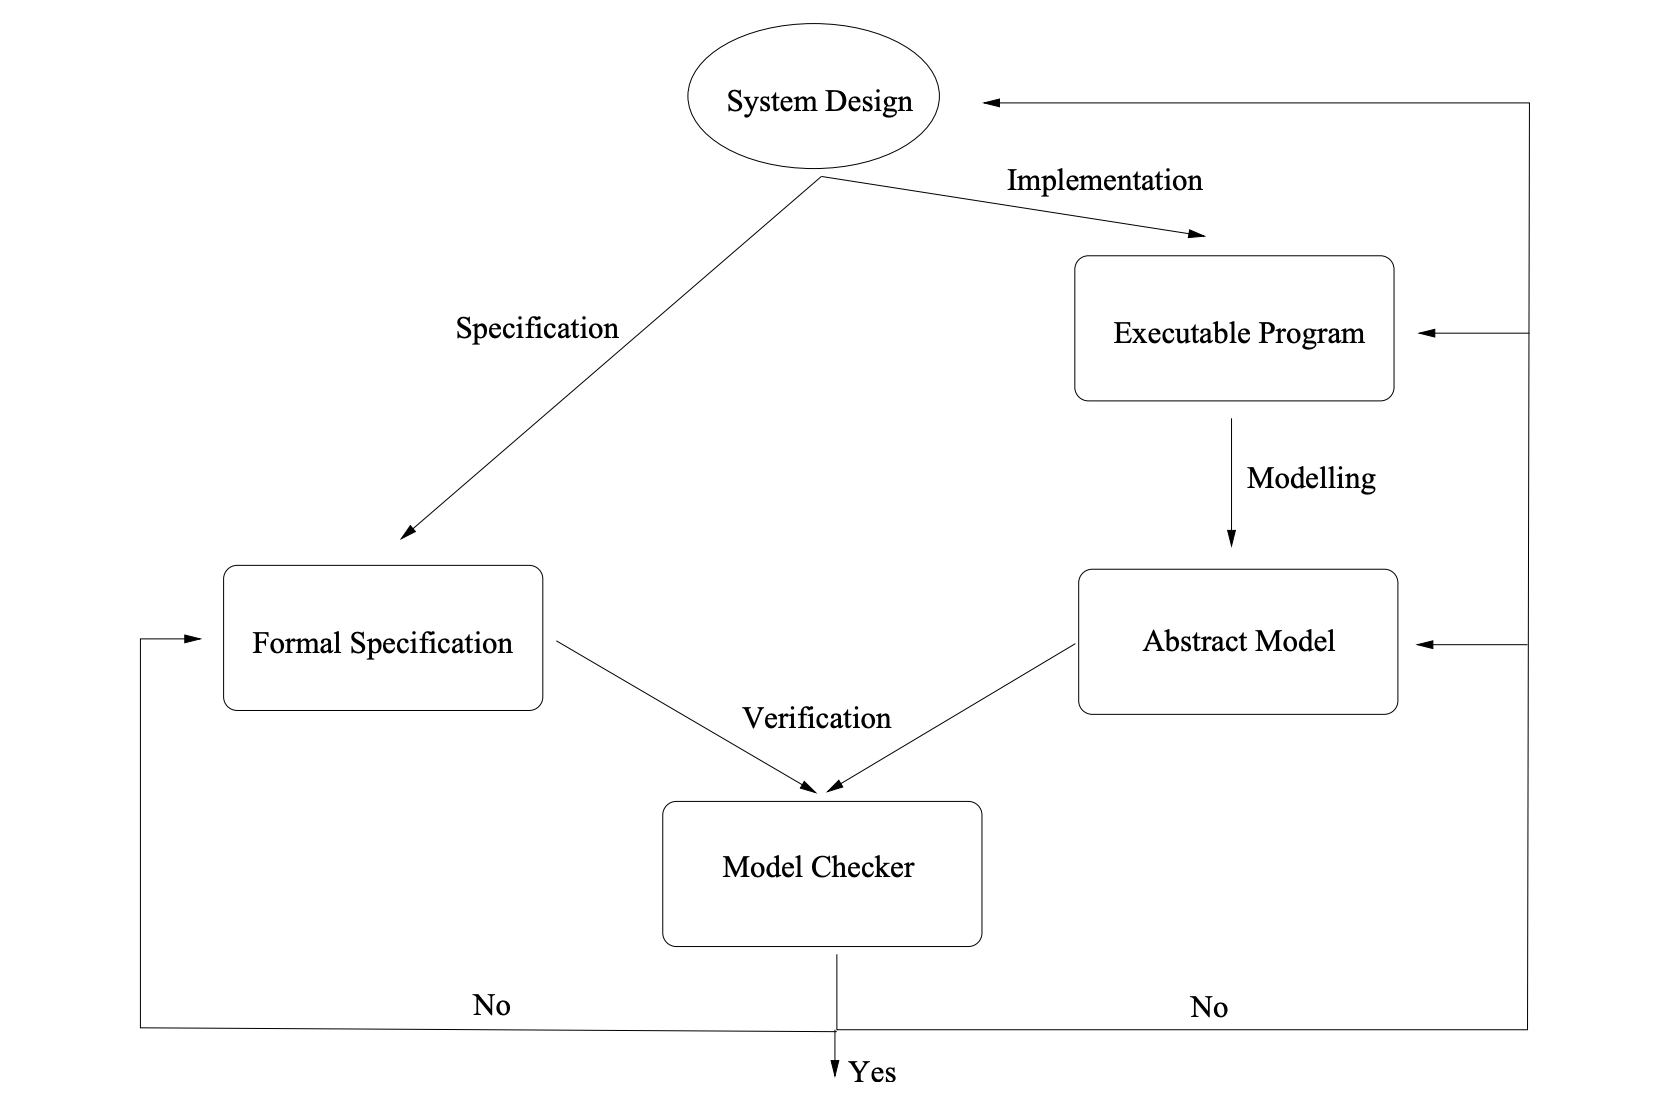
\includegraphics[width=1.0\textwidth]{Immagini/the_process_of_model_checking.jpg}
	\caption{The process of model checking \cite{ModelCheckingProcess}}
	\label{fig:one}
\end{figure}
It is important to pay particular attention to the modeling and specification phases, since errors can make this method give false positives.
Having said that, model checking is a precious method used in several static analysis tools. 

\section{Constraint satisfaction}
Constraint satisfaction is the process of finding a solution through a set of constraints that impose conditions some variables must satisfy.
It is one of the subjects of investigation in the fields of artificial intelligence and operations research.

In particular, Constraint Satisfaction Problems (CSPs) form a specific class of search problems. A CSP is a triple which comprehend:
\begin{itemize}
  \item variables, a finite and non empty set;
  \item domains, finite and non empty sets, one for each variable;
  \item constraints over variables, such that each constraint is a subset of the cartesian product of domains sets.
\end{itemize}
Solutions are combinations of values that can be assigned to the variables, from the respective domains, that satisfies all the constraints at the same time.
\\\\
Constraint satisfaction has also been used to perform checks on programs during static analysis.
Constraint propagation is an essential part of this method, which, relying on local consistency conditions, tries to reduce domains of variables, strengthen constraints, or create new ones. 
To give an idea about the possible use cases of such an approach let's consider an example found in ``A Practical Approach to Verification of Floating-Point C/C++ Programs'' by Bagnara et al. \cite{10.1145/3410875}. 
In Chapter 3 the expression
\begin{quote}
\itshape
float phi\textunderscore = asin(sin(dl) / cosh(ll));
\end{quote}
is translated into static single assignment form and is decomposed. We can read about this:
\begin{quote}
\itshape
``In this intermediate code representation, complex expressions are decomposed into sequences of assignment instructions where at most one operator is applied, and new variable names are introduced so that each variable is assigned to only once.''
\end{quote}
The expression results in a list of statements like this:
\begin{lstlisting}
float phi_; double z1, z2, z3, z4, z5, z6;
z1 = (double) dl;
z2 = sin(z1);
z3 = (double) ll;
z4 = cosh(z3);
z5 = z2/z4;
z6 = asin(z5);
phi_ = (float) z6;	
\end{lstlisting}
and then, regarding line 6:
\begin{quote}
\itshape
``Let us see how this can be used for program verification. As a first example, let us consider the question of whether the division z5 = z2 / z4 can give rise to a division by zero. Assume that all of the intervals are initially full - for instance, they contain all possible numerical floating-point values and all propagators are ready to run. We modify the interval associated to z4 to [-0, +0] and start propagation. At some stage, the indirect propagator for cosh will be called to possibly refine the interval for z3 starting from the interval of z4: a propagator correctly capturing a passable implementation of cosh will refine the label of z3 to the empty interval, thus proving that division by zero is indeed not possible.''
\end{quote}

\section{MISRA C}
MISRA C is a set of software development guidelines and the de facto standard for developing software in C where safety, security and code quality are important. 
It was originally developed to fulfill the need for a ``restricted subset of a standardized programming language'' identified in the 1994 ``Development guidelines for vehicle based software'' and against the background of the emerging use of C for developing embedded software in automotive applications.
Although originally specifically targeted at the automotive industry, it has evolved as a widely accepted model for best practices by leading developers in sectors including automotive, aerospace, telecom, medical devices, defense, railway, and others.
MISRA standards are used to ensure that the code is:
\begin{itemize}
  \item safe;
  \item secure;
  \item reliable;
  \item portable.
\end{itemize}
As we can read in ``A Rationale-Based Classification of MISRA C Guidelines'', Bagnara et al \cite{BagnaraBH22}:
\begin{quote}
\itshape
``Each of the 175 guidelines of MISRA C is classified as being either a \textbf{directive} or a \textbf{rule}:
\\
\textbf{Rule}: a guideline such that information concerning compliance is fully contained in the source code and in the language implementation.
\\
\textbf{Directive}: a guideline such that information concerning com- pliance is not fully contained in the source code and language implementation: requirements, specifications, designs and other considerations may need to be taken into account.

One of the things that is often misunderstood is that MISRA C is much more than just the set of its guidelines. The guidelines are meant to be used in the framework of a documented software development process.
\\\\
...
\\\\
The \textbf{deviation process} is an essential part of the adoption of the MISRA Guidelines, each one of which is assigned a single category: \textbf{mandatory}, \textbf{required} or \textbf{advisory}, defined as follows.

\textbf{Mandatory}: C code that complies with MISRA C must comply with every mandatory guideline: deviation is not permitted.

\textbf{Required}: C code that complies with MISRA C shall comply with every required guideline: a formal deviation is required where this is not the case.

\textbf{Advisory}: these are recommendations that should be followed as far as it is reasonably practical: formal deviation is not required, but non-compliances should be documented.

Whenever complying with a guideline goes against code quality or does not allow access to the hardware or does not allow integrating or use suitably qualified adopted code, the guideline has to be deviated. That is, instead of modifying the code to bring it into compliance, for required guidelines, a written argument has to be provided to justify the violation whereas, for advisory guidelines, this is not necessary.''
\end{quote}
MISRA comprehends a number of rules that are focused mainly on these aspects:
\begin{itemize}
  \item avoiding possible compiler differences;
  \item avoiding using functions and constructs that are prone to failure;
  \item produce maintainable and debuggable code;
  \item best practices in general;
  \item complexity limits.
\end{itemize}
At the moment of this writing there have been three releases of the MISRA C standard:
\begin{itemize}
  \item MISRA C:1998;
  \item MISRA C:2004;
  \item MISRA C:2012.
\end{itemize}
A small selection from the MISRA C 2012 guidelines follows, in order to convey the overall idea of the coding standard:

\noindent\rule{\textwidth}{0.1pt}

\emph{Rule 15.6}:\\

\noindent\fbox{%
    \parbox{\textwidth}{%
      The body of an iteration-statement or a selection-statement shall be a compound-statement
    }%
}
\\\\
\textbf{Category}: Required\\
\textbf{Analysis}: Decidable, Single Translation Unit\\
\textbf{Applies to}: C90, C99\\

It is possible for a developer to mistakenly believe that a sequence of statements forms the body of an iteration-statement or selection-statement by virtue of their indentation. The accidental inclusion of a semi-colon after the controlling expression is a particular danger, leading to a null control statement. Using a compound-statement clearly defines which statements actually form the body.
Additionally, it is possible that indentation may lead a developer to associate an else statement with the wrong if.
\\\\
A famous case in which such a rule would have prevented problems is the ``Apple goto fail vulnerability'': 
on 2014-02-21 Apple released a security update for its implementation of SSL/TLS in many versions of its operating system 
and the indicted code is reported in Listing~\ref{lst:the-apple-goto-fail-vuln}.
\begin{quote}
\itshape
``The problem was the second (duplicate) ``goto fail''. 
The indentation here is misleading; since there are no curly braces after the ``if'' statement, the second ``goto fail'' is always executed. In context, that meant that vital signature checking code was skipped, so both bad and good signatures would be accepted. The extraneous ``goto'' caused the function to return 0 (``no error'') when the rest of the checking was skipped; as a result, invalid certificates were quietly accepted as valid.'' \cite{TheAppleGotoFailVulnerability}
\end{quote}

\begin{lstlisting}[caption={The Apple goto fail vulnerability}, label={lst:the-apple-goto-fail-vuln}]
if ((err = SSLHashSHA1.update(&hashCtx, &signedParams)) != 0)
  goto fail;
  goto fail;
... other checks ...
fail:
  ... buffer frees (cleanups) ...
  return err;
\end{lstlisting}

\noindent\rule{\textwidth}{0.1pt}

\emph{Rule 3.2}:\\

\noindent\fbox{%
    \parbox{\textwidth}{%
    Line-splicing shall not be used in // comments
    }%
}
\\\\
\textbf{Category}: Required\\
\textbf{Analysis}: Decidable, Single Translation Unit\\
\textbf{Applies to}: C99\\

If a // commented line ends with a back-slash followed by a new-line, then the following line is part of the comment, and, if this was not intended, an important line of code maybe lost. 
The following example shows how a seemingly-innocuous path separator at the end of the comment may accidentally comment out the next line of code. \cite{BagnaraBH18}

\begin{lstlisting}[caption={Examples of MISRA C 2012 Rule 3.2 violation and compliance}]
// see critical.* in c:\project\src\
critical_function(); /* Non-compliant */

// see critical.* in c:\project\src
critical_function(); /* Compliant */
\end{lstlisting}

\clearpage

\emph{Rule 9.1}:\\

\noindent\fbox{%
    \parbox{\textwidth}{%
    The value of an object with automatic storage duration shall not be read before it has been set
    }%
}
\\\\
\textbf{Category}: Mandatory\\
\textbf{Analysis}: Undecidable, System\\
\textbf{Applies to}: C90, C99\\

Note that array elements and structure members are considered as discrete objects and they must be (recursively) initialized. 
The rationale is that, according to the C Standard, objects with automatic storage duration are not automatically initialized and can therefore have indeterminate values. Reading them while their value is indeterminate is undefined behavior. \cite{BagnaraBH18}

\noindent\rule{\textwidth}{0.1pt}

\emph{Dir 4.4}:\\

\noindent\fbox{%
    \parbox{\textwidth}{%
      Sections of code should not be ``commented out''
    }%
}
\\\\
\textbf{Category}: Advisory\\
\textbf{Applies to}: C90, C99\\

This rule applies to both // and /* ... */ styles of comment.
Where it is required for sections of source code not to be compiled then this should be achieved by use of conditional compilation (e.g. \#if or \#ifdef constructs with a comment). Using start and end comment markers for this purpose is dangerous because C does not support nested comments, and any comments already existing in the section of code would change the effect.